\documentclass[11pt]{article}

\usepackage{sympytex}
\usepackage{parskip}
\usepackage{subcaption}
\usepackage{graphicx}
\usepackage{multicol}

\usepackage{cancel}
\usepackage{centernot}
\usepackage[table]{xcolor}
\usepackage{booktabs}
%\usepackage{tabularray}

\usepackage{amsmath}
\usepackage{amsthm}
\usepackage{physics}
\usepackage{amsfonts}
\usepackage{amssymb}
\usepackage{mathtools}
\usepackage{esvect}
\usepackage{bm}

\usepackage{surround}
\usepackage{emnotation}

\usepackage{hyperref}
\hypersetup{
    colorlinks=true,
    linktoc=all,
    linkcolor=black,
    urlcolor=blue
}

\setcounter{secnumdepth}{4}
\setcounter{tocdepth}{5}

\topmargin=-0.45in
\evensidemargin=0in
\oddsidemargin=0in
\textwidth=6.5in
\textheight=9.0in
\headsep=0.25in

\setlength\parindent{0pt}
\setlength\parskip{6pt}

\linespread{1.1}

\title{Signals and Systems Quick Reference \\ Revision 0.3}
\author{Emmy Chow}
\date{}

\begin{document}
  \maketitle
  \tableofcontents

  \pagebreak

  \section{Notation and Definitions}

  \subsection{Notation}

  \subsubsection{Logic}

  \(:= \) means equal by definition

  \(\contra\) means contradiction
  \subsubsection{Set Definitions}

  \textbf{Topology and Basic Sets}

  \(\partial U\) is the boundary of \(U\)

  \(\overbar{U}\) is the closure of \(U\). i.e. a set plus its boundary.

  \(\interior{U}\) is the interior of \(U\) i.e. a set plus minus its boundary.

  \(\abs{U}\) is the size or \href{https://www.wikiwand.com/en/Cardinality}{cardinality} of set \(U\)

  \(\mathbb{N} := \displaystyle \bigcup_{k = 1}^{\infty} \{k\}\) is the set of natural numbers

  \(\mathbb{N}_0 := \mathbb{N} \cup \{0\}\) is the set of whole numbers

  \(\mathbb{R}_{+} := \brc{x \in \mathbb{R} : x > 0}

  \(|\mathbb{N}| = \aleph_0\)

  \textbf{Subsets of} \(\mathbb{Z}\) \textbf{and} \(\mathbb{N}_0\)

  Given \(k, a \in \mathbb{Z}\),
  \(k\mathbb{Z} + a:= \brc{kn + a : n \in \mathbb{Z}} = \brc{a, -k + a, k + a, 2k + a, -2k + a, \dots}\)

  Given \(k, a \in \mathbb{N}_0\),
  \(k\mathbb{N}_0 + a:= \brc{kn + a : n \in \mathbb{N}_0} = \brc{a, k + a, 2k + a, 3k + a, \dots}\)

  I extend interval notation to the integers. Instead of a comma, two dots are used between the upper and lower bound when it's set
  of integers. For example: \([a\,..\,b) := [a, b) \cap \mathbb{Z}\).

  \textbf{Other Set definitions}

  \(\mathbb{F}\) is a general field. It can be either \(\mathbb{R}\) or \(\mathbb{C}\)

  \(\overbar{\mathbb{C}} := \mathbb{C} \cup \{\infty\}\) is the \href{https://www.wikiwand.com/en/Riemann_sphere}{Riemann Sphere}

  \(\brc{a_i}_{i = k}^n := \brc{a_i}_{i \in [k\,..\,n]}\) is an \href{https://www.wikiwand.com/en/Index_set}{indexed set}.
  Informally, for indexed sets \(\brc{a_1, a_2} \neq \brc{a_2, a_1}\).

  \textbf{Algebraic Structure}

  \(\prn{V,\, \mathbb{F}}\) is a vector space

  \(\prn{V,\, \mathbb{F}, \norm{\cdot}}\) is a metric space

  \(\prn{V,\, \mathbb{F}, \innerprod{\cdot,\, \cdot}}\) is an inner product space

  \(U \le W\) means \(U\) is a vector subspace of \(W\)

  \(U < W\) means \(U\) is a proper vector subspace of \(W\)

  \pagebreak

  \subsubsection{Linear Algebra}

  \([0]\) is the matrix with all entries equal to \(0\)

  \(\bm{A} \sim \bm{B}\) means \(\bm{A}\) is row equivalent to \(\bm{B}\)

  \(\diag{a_i}_{i = 1}^n :=
  \begin{bmatrix} a_1 & \dots & a_n\end{bmatrix} \bm{I}\)

  \(\displaystyle \bigoplus_{i = 1}^n \bm{A}_k = \bm{A}_1 \oplus \cdots \oplus \bm{A}_n := \diag{\bm{A_1}, \cdots, \bm{A}_n}\)

  \vspace{12pt}

  \textbf{Basis Representation}

  \(\mathcal{E}_U := \brc{\vu{u}_i}_{i = 1}^n\) is the standard basis for \(U\)

  \(\mathcal{B}_U := \brc{\vect{u}_i}_{i = 1}^n\) is a basis for \(U\)

  \(\bkt{\mathcal{B}_U}\) is the matrix with columns corresponding to elements of the basis \(\mathcal{B}_U\)

  \(\mathcal{E}_n := \brc{\vect{e}_i}_{i = 1}^n\) is the standard basis for \(\mathbb{R}^n\)

  \(\vect{x}_{\mathcal{B}_U}\) is the vector \(\vect{x} \in U\) wrt basis \(\mathcal{B}_U\)

  \(\bm{P}_{\mathcal{B}_U \to \mathcal{B}_W} := \bkt{\mathcal{B}_U}^{-1}\bkt{\mathcal{B}_W}\) is the change of basis matrix
  from basis \(\mathcal{B}_U\) to basis \(\mathcal{B}_W\)

  \(\mathfrak{L}(U, W)\) is the set of linear operators that maps
  \((U, \mathbb{F})\) to \((W, \mathbb{F})\)

  \(\bkt{\mathcal{T}}_{(\mathcal{B}_U,\, \mathcal{B}_W)}\) is the matrix representation of linear operator \(\mathcal{T}\)
  with vectors in the domain wrt \(\mathcal{B}_U\) and vectors in the codomain
  wrt \(\mathcal{B}_W\)

  \vspace{12pt}

  \textbf{Eigenvalues and Eigenvectors}

  \(\charc{\bm{A}}(\lambda) := \det{\bm{A} - \lambda\bm{I}}\)

  \(\spec{\bm{A}}\) is the spectrum (set of all eigenvalues) of \(\bm{A}\).

  \(\minpoly{\bm{A}}(\lambda)\) is the minimal polynomial for the matrix \(\bm{A}\)

  \(\alg{\bm{A}}(\lambda)\) is the algebraic multiplicity of eigenvalue \(\lambda\) for the matrix \(\bm{A}\)

  \(\geom{\bm{A}}(\lambda)\) is the geometric multiplicity of eigenvalue \(\lambda\) for the matrix \(\bm{A}\)

  \vspace{12pt}

  \textbf{Definiteness}

  \(\bm{A} \succ 0 \iff \) \(\bm{A}\) is positive definite,

  \(\bm{A} \succeq 0 \iff\) \(\bm{A}\) is positive semidefinite

  \(\bm{A} \prec 0 \iff \) \(\bm{A}\) is negative definite,

  \(\bm{A} \preceq 0 \iff\) \(\bm{A}\) is negative semidefinite

  \pagebreak

  \subsubsection{Calculus}

  \begin{multicols}{2}
  \textbf{Nth Derivative/Antiderivative}

  \(\D^nf(t) := f^{(n)}(t)\) \\

  \(\D^{-n}f(t) := \underbrace{\displaystyle
  \int \cdots \int}_{\textrm{n times}}{f(t)\,dt \dots dt}\)

  \columnbreak

  \textbf{Accumulation}

  \(\A^{k}f(t) := \underbrace{\intlim{-\infty}{t} \cdots \intlim{-\infty}{t}}_{\textrm{k times}}{f(\tau)\,d\tau \cdots d\tau}\)

  \(\A^{k}f[n] := \displaystyle
  \underbrace{\sum_{n = -\infty}^n \dots \sum_{k = -\infty}^n}_{\textrm{k times}}f[k]\)

  \end{multicols}

  \textbf{Jacobian and Parital Derivatives:}

  \(\partial^n_{x_{_1}}f(x_1, \dots, x_n) := \dfrac{\partial^n f}{\partial x^n}\)

  \vspace{12pt}

  \(\partial^{-n}_{x_{_1}}f := \underbrace{\int \dots \int}_{\textrm{n times}}{f(x_1, \dots, x_n)\,dx_1 \cdots dx_1}\)

  \vspace{12pt}

  If mixed partials commute we can write:

  \(\partial^{(k_1,\, \dots,\, k_n)}_{x_{_1},\, \dots,\, x_{_k}}f(x_1, \dots, x_n) :=
  \dfrac{\partial^K f}{\partial x_1^{k_1} \cdots \partial x_n^{k_n}}\), where \(K = k_1 + \dots + k_n\)


  \(\bkt{\D \vect{f}(x_1, \dots, x_n)} =
  \begin{bmatrix}
    \partial_{x_{_1}} \vect{f} & \dots & \partial_{x_{_n}} \vect{f}
  \end{bmatrix} :=
  \begin{bmatrix}
    \partial_{x_{_1}} f_1 & \dots & \partial_{x_{_n}} f_1 \\
    \vdots & \ddots & \vdots \\
    \partial_{x_{_1}} f_n & \dots &  \partial_{x_{_n}} f_n
  \end{bmatrix}\)

  \subsubsection{Complex Numbers}

  \((a + bj)^* := a - bj\) is the complex conjugate

  \(\Re{a + bj} := a\)

  \(\Im{a + bj} := b\)

  \(\bm{A}^{\H} := (\bm{A}^*)^\T = \prn{\bm{A}^\T}^*\)

  \pagebreak

  \subsubsection{Linear Systems Theory}


  \pagebreak

  \subsubsection{Digital Signal Processing}

  \textbf{Delta Operator}

  \(\Delta x[n] := x[n + 1] - x[n]\)

  \(\Delta^k x[n] := \Delta^{k - 1} x[n + 1] - \Delta^{k - 1}x[n]\)

  \vspace{12pt}

  \textbf{Circular Convolution}

  \(f(t) \oast g(t) :=
  \intlim{\theta_0}{\theta_0 + 2\pi} f(\tau)g(t - \tau)\,d\tau\),
  \(\theta_0 \in \mathbb{R}\)

  \vspace{12pt}

  \textbf{Useful Functions/Equations:}

  \(\sgn(x) := \begin{cases}
    1 \IF x > 0 \\
    0 \IF x = 0 \\
    -1 \IF x < 0 \\
  \end{cases}\)

  \(\displaystyle \clamp_{[a,\, b]}(x) := \min(\max(x, a), b)\)

  \(\Arg(\theta) := \theta  - 2\pi\floor{\dfrac{\theta - \theta_0}{2\pi}}\)
  (i.e. \(\theta \in \mathbb{R}\) maps to \(\hat{\theta} \in [\theta_0,\, \theta_0 + 2\pi]\))


  \pagebreak

  \subsection{Function Definitions}

  \bgroup
  \rowcolors{2}{gray!10}{gray!30}
  \renewcommand{\arraystretch}{2.4}
  \setlength{\tabcolsep}{0.8cm}
  \large\begin{tabular}{c|c}
    Name & Definition \\
    \hline
    (Heaviside) unit step function &
      \(u_{H}(t) := \begin{cases} 1 \textrm{ if }  x > 0  \\ 0, \textrm{ otherwise}  \end{cases}\) \\
    Discrete rectangular function & \(\rect[x] := u_{H}[x] - u_{H}[x - 1]\) \\
    Discrete Triangular function & \(\tri[n] :=
    (1 - |x|)\rect\bkt{\frac{1}{2}(x + 1)}\) \\
    Continuous rectangular function & \(\rect(x) := u_H\prn{x + \frac{1}{2}} - u_H\prn{x - \frac{1}{2}}\) \\
    Triangular function & \(\tri(x) :=
    (1 - |x|)\rect\prn{\frac{1}{2}x}\) \\
    ReLU/Ramp function & \(\relu(x) := u_H(x)x\) \\
    (Normalized) sinc & \(\sinc(x) := \dfrac{\sin(\pi x)}{\pi x}\) \\
    Dirichlet kernel & \(\diric_N(x) := \dfrac{\sin\prn{\prn{N + \frac{1}{2}}x}}{\sin\prn{\frac{x}{2}}}\) \\
    (Dirac) comb function & \(W_T(x) := \displaystyle \sum_{k = -\infty}^\infty \delta(t - kT)\) \\
  \end{tabular}
  \egroup

  \vspace{12pt}

  Note:

  Discrete functions can only be scaled by integer factors.

  \pagebreak

  \section{Identities}

  \subsection{Trig Identities}

  \begin{multicols}{2}
  \textbf{Co-Function Identities} \\
  \({\cos}\prn{\frac{\pi}{2} - \theta} = \sin(\theta)\)\vspace{6pt} \\
  \({\sin}\prn{\frac{\pi}{2} - \theta} = \cos(\theta)\) \vspace{6pt} \\
  \({\tan}\prn{\frac{\pi}{2} - \theta} = \cot(\theta)\) \\
  %\(\sec\prn{\frac{\pi}{2} - \theta} = \csc(\theta)\) \vspace{6pt} \\
  %\(\csc\prn{\frac{\pi}{2} - \theta} = \sec(\theta)\) \vspace{6pt} \\
  %\(\cot\prn{\frac{\pi}{2} - \theta} = \tan(\theta)\) \\\\

  \textbf{Supplement Angle Identities} \\
  \(\sin(\pi - \theta) = \sin(\theta)\) \\
  \(\sin(\pi + \theta) = -\sin(\theta)\)\vspace{6pt} \\
  \(\cos(\pi - \theta) = -\cos(\theta)\) \\
  \(\cos(\pi + \theta) = -\cos(\theta)\)\vspace{6pt} \\
  \(\tan(\pi - \theta) = -\tan(\theta)\) \\
  \(\tan(\pi + \theta) = \tan(\theta)\) \\

  \textbf{Negative Angle Identities}\\
  \(\sin(-\theta) = -\sin(\theta)\) \vspace{6pt} \\
  \(\cos(-\theta) = \cos(\theta)\) \vspace{6pt} \\
  \(\tan(-\theta) = -\tan(\theta)\) \\
  %\(\sec(-\theta) = \sin(\theta)\) \vspace{6pt} \\
  %\(\csc(-\theta) = -\csc(\theta)\) \vspace{6pt} \\
  %\(\cot(-\theta) = -\cot(\theta)\) \vspace{6pt} \\\\

  \textbf{Additional and Subtraction Identities}\\
  \(\sin(x + y) = \sin(x)\cos(y) + \cos(x)\sin(y)\) \vspace{6pt} \\
  \(\sin(x - y) = \sin(x)\cos(y) - \cos(x)\sin(y)\) \vspace{6pt} \\
  \(\cos(x + y) = \cos(x)\cos(y) - \sin(x)\sin(y)\) \vspace{6pt} \\
  \(\cos(x - y) = \cos(x)\cos(y) + \sin(x)\sin(y)\) \\

  \textbf{Product Identities}\\
  \(\sin(x)\cos(y) = \frac{1}{2}(\sin(x + y) + \sin(x - y))\) \vspace{6pt}\\
  \(\cos(x)\sin(y) = \frac{1}{2}(\sin(x + y) - \sin(x - y))\) \vspace{6pt}\\
  \(\cos(x)\cos(y) = \frac{1}{2}(\cos(x + y) - \cos(x - y))\) \vspace{6pt}\\
  \(\sin(x)\sin(y) = \frac{1}{2}(\cos(x - y) - \cos(x + y))\) \\

  \textbf{Superposition}\\
  \(A_1\cos(\theta) + A_2\sin(\theta) = A\,{\cos}\prn{\theta - \phi}\)

  \(A = \sqrt{A_1^2 + A_2^2}\,\),
  \(\phi = {\tan^{-1}}\prn{\dfrac{A_2}{A_1}}\)

  \columnbreak

  \textbf{Power Reduction Formula}\\
  \(\sin^2(\theta) = \frac{1}{2}(1 - \cos(2\theta))\) \vspace{6pt}\\
  \(\cos^2(\theta) = \frac{1}{2}(1 + \cos(2\theta))\) \\

  \textbf{Double Angle Identities}\\
  \(\sin(2\theta) = 2\sin(\theta)\cos(\theta)\) \\
  \(\cos(2\theta) = \cos^2(\theta) - \sin^2(\theta)\) \\
  \(\textrm{ }\textrm{ }\textrm{ }\textrm{ }\textrm{ }\textrm{ }\textrm{ }\textrm{ }\textrm{ }\,
  = 2\cos^2(\theta) - 1\) \\
  \(\textrm{ }\textrm{ }\textrm{ }\textrm{ }\textrm{ }\textrm{ }\textrm{ }\textrm{ }\textrm{ }\,
  = 1 - 2\sin^2(\theta)\) \vspace{6pt} \\
  \(\tan(2\theta) = \dfrac{2\tan(\theta)}{1 - \tan^2(\theta)}\)
  \vspace{6pt}\\

  \textbf{Half Angle Identities}\\
  \(\sin\prn{\dfrac{\theta}{2}} = \pm \sqrt{\dfrac{1 - \cos(\theta)}{2}}\) \vspace{6pt}\\
  \(\cos\prn{\dfrac{\theta}{2}} = \pm \sqrt{\dfrac{1 + \cos(\theta)}{2}}\) \vspace{6pt}\\

  \textbf{Sum Identities}\\
  \(\sin(x) + \sin(y) = 2\sin\prn{\dfrac{x + y}{2}}\cos\prn{\dfrac{x - y}{2}}\) \vspace{10pt}\\
  \(\sin(x) - \sin(y) = 2\cos\prn{\dfrac{x + y}{2}}\sin\prn{\dfrac{x - y}{2}}\) \vspace{10pt}\\
  \(\cos(x) + \cos(y) = 2\cos\prn{\dfrac{x + y}{2}}\cos\prn{\dfrac{x - y}{2}}\) \vspace{10pt}\\
  \(\cos(x) - \cos(y) = 2\cos\prn{\dfrac{x + y}{2}}\cos\prn{\dfrac{x - y}{2}}\) \vspace{10pt}\\
  \textbf{Complex Exponential Identities}\\
  \(\sin(z) = \dfrac{1}{2j}\prn{e^{jz} - e ^{-jz}}\)\vspace{6pt}\\
  \(\cos(z) = \dfrac{1}{2}\prn{e^{jz} + e ^{-jz}}\)
  \end{multicols}

  \pagebreak

  \subsection{Other Identities}


  \textbf{Convolutions}

  \(f(x) \star g(x) = f(x) * g(-x)\)

  \(\rect(x) * \rect(x) = \tri(x)\)

  \vspace{12pt}

  \textbf{Dirichlet Kernel}

  \(\displaystyle
  \diric_N(x) := \dfrac{\sin(\prn{n + \frac{1}{2}}x)}{\sin\prn{\frac{x}{2}}} =
  \sum_{k = -N}^{N} e^{jkx} =
  1 + 2\sum_{k = 1}^N\cos(kx)\)

  \(\displaystyle \lim_{N \to \infty} \diric_{N}(Tx) = W_{\frac{1}{T}}(x)\)

  \textbf{Accumulation}

  \(\mathcal{A}\brc{\Delta x[t]} = \Delta\brc{\mathcal{A} x[t]} = x[t]\)

  \(\mathcal{A}\brc{\D x(t)} = \D\brc{\mathcal{A} x(t)} = x(t)\)

  \pagebreak

  \section{Linear Systems Theory}

  \subsection{Continuous Time Fourier Transform}

  \begin{multicols}{2}
    \(X\prn{e^{j\omega}} = \F\brc{x(t)} := \intlim{-\infty}{\infty} x(t)e^{-j\omega t}\, dt\)

    \columnbreak

    \(x(t) = \F^{-1}\brc{X\prn{e^{j\omega}}} := \dfrac{1}{2\pi}\intlim{-\infty}{\infty} X\prn{e^{j\omega}}e^{j\omega t} d\omega\)
  \end{multicols}

  \subsubsection{CTFT Properties}

  \bgroup
  \rowcolors{2}{gray!10}{gray!30}
  \renewcommand{\arraystretch}{2.1}
  \setlength{\tabcolsep}{0.55cm}
  \large\begin{tabular}{c|c|c}
    Property & Time Domain & Frequency Domain \\
    \toprule
    Linearity & \(c_1x_1(t) + c_2x_2(t)\) & \(c_1X_1\prn{e^{j\omega}} + c_2X_2\prn{e^{j\omega}}\) \\
    Time Shift & \(x(t - t_0)\) & \(X\prn{e^{j\omega}}e^{-j\omega t_0}\)\\
    Time Reversal & \(x(-t)\) & \(X\prn{e^{-j\omega}}\)\\
    Time Scale & \(x(at)\) & \(\dfrac{1}{|a|}X\prn{e^{\frac{j\omega}{a}}}e^{-\frac{j\omega}{a}}\)\\
    Time Scale + Shift & \(x(at - t_0)\) & \(\dfrac{1}{|a|}X\prn{e^{\frac{j\omega}{a}}}e^{-\frac{j\omega t_0}{a}}\)\\
    Complex Conjugation & \(x^*(t)\) & \(X^*\prn{e^{-j\omega}}\)\\
    Frequency Shift & \(x(t)e^{-j\omega_0}\) & \(X\prn{e^{j(\omega - \omega_0)}}\)\\
    Convolution & \(x_1(t) * x_2(t)\) & \(X_1\prn{e^{j\omega}}X_2\prn{e^{j\omega}}\) \\
    Modulation & \(x_1(t)x_2(t)\) & \(\dfrac{1}{2\pi}X_1\prn{e^{j\omega}} * X_2\prn{e^{j\omega}}\) \\
    Time Differentiation & \(\D_t^n\{x(t)\}\) & \((j\omega)^nX\prn{e^{j\omega}}\) \\
    Causal Accumulation &
    \(\A_t\{x(t)u_H(t)\}\) & \(\dfrac{1}{j\omega}X\prn{e^{j\omega}} + \pi X(0)\delta(\omega)\) \\
    Frequency Differentiation & \(t^n x(t)\) & \(j^n\D_{\omega}^n\{X\parenf{e^{j\omega}}\}\) \\
    Parseval's Theorem & \(\displaystyle\int_{-\infty}^{\infty} x_1(t)x^*_2(t)\,dt \) &
    \(\dfrac{1}{2\pi}\displaystyle\int_{-\infty}^{\infty} X_1\prn{e^{j\omega}}X_2^*\prn{e^{j\omega}} \,d\omega\) \\
    Duality & \(X\prn{e^{j\omega t}}\) & \(2\pi x\prn{\omega}\)
  \end{tabular}
  \egroup

  \pagebreak

  \subsubsection{CTFT Table}

  \bgroup
  \rowcolors{2}{gray!10}{gray!30}
  \renewcommand{\arraystretch}{1.8}
  \setlength{\tabcolsep}{1.7cm}
  \normalsize\begin{tabular}{c|c}
    \(f(t)\) & \(F\prn{e^{j\omega}}\) \\
    \toprule
    \(0\) & constant \(\omega_0\) \\
    \(1\) & \(2\pi\delta\prn{\omega}\) \\
    \(\delta(t)\) & \(1\) \\
    \(u(t)\) & \(\pi\delta(\omega) + \dfrac{1}{j\omega}\) \\
    \(\sgn(t)\) & \(\dfrac{2}{j\omega}\) \\
    \(e^{j\omega_0t}\) & \(2\pi\delta(\omega - \omega_0)\) \\
    \(\cos(\omega_0t)\) & \(\pi\prn{\delta(\omega - \omega_0) + \delta(\omega + \omega_0)}\) \\
    \(\sin(\omega_0t)\) & \(-j\pi\prn{\delta(\omega - \omega_0) - \delta(\omega + \omega_0)}\) \\
    \(\cos(\omega_0)u(t)\) & \(\dfrac{\pi}{2}\prn{\delta(\omega - \omega_0) + \delta(\omega + \omega_0)} +
    \dfrac{j\omega}{\omega_0^2 -  \omega^2}\) \\
    \(\sin(\omega_0)u(t)\) & \(\dfrac{\pi}{2j}\prn{\delta(\omega - \omega_0) + \delta(\omega + \omega_0)} +
    \dfrac{\omega_0}{\omega_0^2 -  \omega^2}\) \\
    \(e^{-at}\cos(\omega_0)u(t)\) & \(\dfrac{\omega_0}{(a + j\omega)^2 + \omega_0^2}\) \\
    \(e^{-at}\sin(\omega_0)u(t)\) & \(\dfrac{a + j\omega}{(a + j\omega)^2 + \omega_0^2}\) \\
    \(\rect\prn{\dfrac{t}{T}}\),\(\ T > 0\) & \(T\sinc\prn{\dfrac{T}{2\pi}\omega}\) \\
    \(\tri\prn{\dfrac{t}{T}}\), \(\ T > 0\) & \(T\sinc^2\prn{\dfrac{T}{2\pi}\omega}\) \\
    \(A\sinc\prn{\dfrac{1}{2\pi A}t}\) & \(\rect\prn{A\omega}\) \\
    \(A\sinc^2\prn{\dfrac{1}{2\pi A}t}\) & \(\tri\prn{A\omega}\) \\
    \(x^n\) & \(2\pi j^n \delta^{(n)}(\omega)\) \\
    \(e^{-at}u(t)\), \(a > 0\) & \(\dfrac{1}{a + j\omega}\) \\
    \(t^ne^{-at}u(t)\), \(a > 0\) & \(\dfrac{1}{(a + j\omega)^{n + 1}}\) \\
    \(e^{-a|t|}\), \(a > 0\) & \(\dfrac{2a}{a^2 + \omega^2}\) \\
    \(e^{-\frac{t^2}{2\sigma^2}}\) & \(\sqrt{2\pi\sigma^2} e^{-\frac{\sigma^2}{2}\omega^2}\) \\
  \end{tabular}
  \egroup

  \pagebreak

  \subsection{Laplace Transform}

  \begin{multicols}{2}
    \(X(s) = \Z\{x(t)\} := \displaystyle \int_{-\infty}^{\infty} x(t)e^{-st}\, dt\)

    \columnbreak

    \(x(t) = \Z^{-1}\{X(s)\} := \displaystyle \int_{-\infty}^{\infty} x(t)e^{-st}\, dt\)
  \end{multicols}

  \subsubsection{Laplace Transform Properties}

  \bgroup
  \rowcolors{2}{gray!10}{gray!30}
  \renewcommand{\arraystretch}{1.8}
  \setlength{\tabcolsep}{0.2cm}
  \normalsize\begin{tabular}{c|c|c}
    Property & \(x[n]\) & \(X(z)\) \\
    \hline
    Linearity & \(c_1x_1(t) + c_2x_2(t)\) & \(c_1X_1(s) + c_2X_2(s)\) \\
    Time Shifting & \(x(t - t_0)u(t - t_0)\) & \(X(s)e^{-st_0}\) \\
    Time Scaling & \(x(at)\) & \(\dfrac{1}{|a|}X\prn{\dfrac{s}{a}}\) \\
    Time Transformation & \(x(at - t_0)u(t - t_0)\) & \(\dfrac{1}{|a|}X\prn{\dfrac{s}{a}}e^{-\frac{st_0}{a}}\) \\
    Frequency Shift & \(e^{at}x(t)\) & \(X(s - a)\) \\
    1st Time Derivative & \(x'(t)\) & \(sX(s) - x(0^-)\) \\
    2nd Time Derivative & \(x''(t)\) & \(s^2X(s) - sx(0^-) - x'(0^-)\) \\
    General Time Derivative (One-Sided) &
    \(\D_t^n\{x(t)u(t)\}\) & \(s^nX(s) - \displaystyle \sum_{k = 1}^{n} s^{n - k}\D_t^{k -1}\{x\}(0^-)\) \\
    General Time Derivative (Two-Sided) &
    \(\D_t^n\{x(t)\}\) & \(s^nX(s)\) \\
    1st Frequency Derivative & \(tx(t)\) & \(-X'(s)\) \\
    General Frequency Derivative & \(t^nx(t)\) & \((-1)^n\D^n_s\{X(s)\}\) \\
    Accumulation & \(\A^n_t\{x(t)\}\) & \(s^{-n}X(s)\) \\
    Frequency Integration & \(\dfrac{1}{t^n}x(t)\) & \(\mathcal{I}^n_{s}\{X(s)\}\) \\
    Convolution & \(x_1(t) * x_2(t)\) & \(X_1(s)X_2(s)\) \\
    Modulation & \(x_1(t)x_2(t)\) & \(\dfrac{1}{2\pi j}
    \displaystyle \lim_{\omega \to \infty}\int_{\sigma - j\omega}^{\sigma + j\omega} X_1(u)X_2(s - u)\,du\) \\
    Complex Conjugation & \(x^*(t)\) & \(X^*(s^*)\) \\
  \end{tabular}

  \textbf{Initial Value Theorem:}

  \(x(t)\) is causal \(\implies x(0^+) = \displaystyle \lim_{s \to \infty} sX(s)\)

  \textbf{Final Value Theorem:}

  \(x(t)\) is causal and stable \(\implies \displaystyle \lim_{t \to \infty} x(t) =\lim_{s \to 0} sX(s)\)

  \pagebreak

  \subsubsection{Laplace Transform Table}

  \bgroup
  \rowcolors{2}{gray!10}{gray!30}
  \renewcommand{\arraystretch}{2}
  \setlength{\tabcolsep}{1.2cm}
  \large\begin{tabular}{c|c|c}
    \(x(t)\) & \(X(s)\) & ROC \\
    \hline
    \(\delta(t)\) & \(1\) & \(\mathbb{C}\) \\
    \(\delta(t - t_0)\) & \(e^{-st_0}\) & \(\mathbb{C}\) \\
    \(u_H(t)\) & \(\dfrac{1}{s}\) & \(\Re{s} > 0\) \\
    \(u_H(t - t_0)\) & \(\dfrac{1}{s}e^{-st_0}\) & \(\Re{s} > 0\) \\
    \(\rect\prn{\dfrac{t}{T}}\) & \(\dfrac{1 - e^{-Ts}}{s}\) & \(\Re{s} > 0\) \\
    \(\relu(t)\) & \(\dfrac{1}{s^2}\) & \(\Re{s} > 0\) \\
    \(t^n u_H(t)\), \(n \in \mathbb{N}_0\) & \(\dfrac{n!}{s^{n + 1}}\) & \(\Re{s} > 0\) \\
    \(t^z u_H(t)\), \(\Re{z} > -1\) & \(\dfrac{\Gamma(z + 1)}{s^{z + 1}}\) & \(\Re{s} > 0\) \\
    \(t^{\frac{1}{n}} u_H(t)\),
    \(n \in \mathbb{N}_0\) & \(\dfrac{\Gamma\prn{\frac{1}{n} + 1}}{s^{\frac{1}{n} + 1}}\) &
    \(\Re{s} > 0\) \\
    \(e^{-at}u(t)\) & \(\dfrac{1}{s + a}\) & \(\Re{s} > -a\) \\
    \(e^{-a|t|}\) & \(\dfrac{2a}{(a^2 - s^2)}\) & \( -a < \Re{s} < a\) \\
    \(\prn{1 - e^{-at}}u(t)\) & \(\dfrac{a}{s(s + a)}\) & \( \Re{s} > 0\) \\
    \(\sin(\omega t)u(t)\) & \(\dfrac{\omega}{s^2 + \omega^2}\) & \( \Re{s} > 0\) \\
    \(\cos(\omega t)u(t)\) & \(\dfrac{s}{s^2 + \omega^2}\) & \( \Re{s} > 0\) \\
    \(e^{-at}\sin(\omega t)u(t)\) & \(\dfrac{\omega}{(s + a)^2 + \omega^2}\) & \(\Re{s} > -a\) \\
    \(e^{-at}\cos(\omega t)u(t)\) & \(\dfrac{s + a}{(s + a)^2 + \omega^2}\) & \(\Re{s} > -a\) \\
  \end{tabular}

  \pagebreak

  \section{Digital Signal Processing}

  \subsection{Discrete Time Fourier Transform}
  \begin{multicols}{2}
    \(X\prn{e^{j\omega}} = \F\brc{x[n]} := \displaystyle \sum_{n = -\infty}^{\infty} x[n]e^{-j\omega n}\)

    \columnbreak

    \(x[n] = \F^{-1}\brc{X\prn{e^{j\omega}}} :=
    \dfrac{1}{2\pi}\intlim{\theta_0}{\theta_0 + 2\pi}
    X\prn{e^{j\omega}}e^{j\omega n} d\omega\)
  \end{multicols}

  \subsubsection{DTFT Properties}

  \bgroup
  \rowcolors{2}{gray!10}{gray!30}
  \renewcommand{\arraystretch}{2.1}
  \setlength{\tabcolsep}{0.8cm}
  \large\begin{tabular}{c|c|c}
    Property & Time Domain & Frequency Domain \\
    \toprule
    Linearity & \(c_1x_1[n] + c_2x_2[n]\) & \(c_1X_1 + c_2X_2\prn{e^{j\omega}}\) \\
    Time Shift & \(x[n - k]\) & \(X\prn{\omega}e^{-j\omega k}\)\\
    Time Reversal & \(x[-n]\) & \(X\prn{e^{-j\omega}}\)\\
    Time Scale & \(x[an]\) & \(\dfrac{1}{|a|}X\prn{e^{\frac{j\omega}{a}}}\)\\
    Time Shift + Scale & \(x[an - k]\) & \(\dfrac{1}{|a|}X\prn{e^{\frac{j\omega}{a}}}e^{-\frac{j\omega k}{a}}\)\\
    Complex Conjugation & \(x^*[n]\) & \(X^*\prn{e^{-j\omega}}\)\\
    Frequency Shift & \(x[n]e^{-j\omega_0}\) & \(X\prn{e^{j(\omega - \omega_0)}}\)\\
    Convolution & \(x_1[n] * x_2[n]\) & \(X_1\prn{e^{j\omega}}X_2\prn{e^{j\omega}}\) \\
    Modulation & \(x_1[n]x_2[n]\) & \(\dfrac{1}{2\pi} X_1\prn{e^{j\omega}} \oast X_2\prn{e^{j\omega}}\) \\
    First Difference & \(\Delta x[n - 1]\) & \(\prn{1 - e^{-j\omega}}X\prn{e^{j\omega}}\) \\
    Accumlation & \(\A_n\{x[n]\}\) & \(\dfrac{1}{1 - e^{-j\omega}}X\prn{e^{j\omega}}\) \\
    Frequency Differentiation & \((-jt)^k x[n]\) & \(\D_{\omega}^k\brc{F\prn{e^{j\omega}}}\) \\
    Parseval's Theorem & \(\displaystyle\sum_{n = -\infty}^{\infty} x_1[n]x_2^*[n] \) &
    \(\dfrac{1}{2\pi}\displaystyle\int_{-\infty}^{\infty} X_1\prn{e^{j\omega}}X_2^*\prn{e^{j\omega}} \,d\omega\) \\
    Duality & \(X(e^{2\pi n})\) & \(2\pi x\prn{-\omega}\)
  \end{tabular}
  \egroup

  \pagebreak

  \subsubsection{DTFT Symmetries}
  \bgroup
  \rowcolors{2}{gray!10}{gray!30}
  \renewcommand{\arraystretch}{2}
  \setlength{\tabcolsep}{1cm}
  \large\begin{tabular}{c|c}
    \(x[n]\) & \(X(z)\)\\
    \toprule
    \(x^*[n]\) & \(X^*\prn{e^{-j\omega}}\) \\
    \(x^*[-n]\) & \(X^*\prn{e^{j\omega}}\) \\
    \(\Re{x[n]}\) & \(X_e\prn{e^{j\omega}}\) \\
    \(j\Im{x[n]}\) & \(X_o\prn{e^{j\omega}}\) \\
    \(x_e[n]\) & \(\Re{X\prn{e^{j\omega}}}\) \\
    \(x_o[n]\) & \(j\Im{X\prn{e^{j\omega}}}\) \\
    Any real \(x[n]\) & \(X\prn{e^{j\omega}} = X^*\prn{e^{-j\omega}}\) \\
    Any real \(x[n]\) & \(\Re{X\prn{e^{-j\omega}}} =
    \Re{X\prn{e^{j\omega}}}\) \\
    Any real \(x[n]\) & \(\Im{X\prn{e^{-j\omega}}} =
    -\Im{X\prn{e^{j\omega}}}\) \\
    Any real \(x[n]\) & \(\abs{X\prn{e^{-j\omega}}} =
    \abs{X\prn{e^{j\omega}}}\) \\
    Any real \(x[n]\) & \(\arg\prn{X\prn{e^{-j\omega}}} =
    -\arg\prn{X\prn{e^{j\omega}}}\) \\
  \end{tabular}
  \egroup

  \pagebreak

  \subsubsection{DTFT Table}

  \bgroup
  \rowcolors{2}{gray!10}{gray!30}
  \renewcommand{\arraystretch}{2}
  \setlength{\tabcolsep}{1.2cm}
  \large\begin{tabular}{c|c}
    \(x[n]\) & \(X\prn{e^{j\omega}}\) \\
    \toprule
    \(0\) & constant \(\omega_0\) \\
    \(1\) & \(2\pi W_{2\pi}(\omega)\) \\
    \(\delta[n]\) & \(1\) \\
    \(u_H[n]\) & \(\dfrac{1}{1 - e^{-j\omega}} + \pi W_{2\pi}(\omega)\) \\
    \(a^n u[n]\), \(|a| < 1\) & \(\dfrac{1}{1 - ae^{-j\omega}}\) \\
    \((n + 1)a^n u[n]\), \(|a| < 1\) & \(\dfrac{1}{\prn{1 - ae^{-j\omega}}^2}\) \\
    \(\dfrac{(n + r - 1)!}{n!(r - 1)!}a^n u[n]\), \(|a| < 1\) & \(\dfrac{1}{\prn{1 - ae^{-j\omega}}^r}\) \\
    \(\rect\bkt{\dfrac{t}{N}}\), \(\ N \in \mathbb{Z}\ \backslash\ \{0\}\) &
      \(\diric_{\frac{N}{2}}(\omega)\) \\
    \(\sinc[\omega_c n]\), \(\omega_c \le \pi\) & \(\rect\prn{\dfrac{1}{\omega_c}\omega}\) \\
    \(e^{j\omega_0 n}\) & \(2\pi W_{2\pi}(\omega - \omega_0)\) \\
    \(\cos[\omega_0 n + \phi]\) & \(\pi e^{j\phi}W_{2\pi}(\omega - \omega_0) + \pi e^{-j\phi}W_{2\pi}(\omega + \omega_0)\) \\
    \(\sin[\omega_0 n + \phi]\) & \(\dfrac{\pi}{j} e^{j\phi}W_{2\pi}(\omega - \omega_0) -
    \dfrac{\pi}{j} e^{-j\phi}W_{2\pi}(\omega + \omega_0)\) \\
  \end{tabular}
  \egroup

  \pagebreak

  \subsection{Z Transform}
  \begin{multicols}{2}
    \(X(z) = \Z\brc{x[n]} := \displaystyle \sum_{n = -\infty}^{\infty} x[n]z^{-n}\)

    \columnbreak

    \(x[n] = \Z^{-1}\brc{X(z)} := \displaystyle \dfrac{1}{2\pi j} \oint_{C} X(z)z^{n - 1}\, dz\)
  \end{multicols}

  \subsubsection{Z Transform Properties}

  \bgroup
  \rowcolors{2}{gray!10}{gray!30}
  \renewcommand{\arraystretch}{2.1}
  \setlength{\tabcolsep}{0.7cm}
  \large\begin{tabular}{c|c|c}
    Property & \(x[n]\) & \(X(z)\) \\
    \hline
    Linearity & \(c_1x_1[n] + c_2x_2[n]\) & \(c_1X_1(z) + c_2X_2(z)\) \\
    Time Shifting & \(x[n - k]\) & \(X(z)z^{-k}\) \\
    Time Reversal & \(x[-n]\) & \(X\prn{z^{-1}}\) \\
    Z-Scaling & \(z_0^nx[n]\) & \(X(z_0^{-1}z)\) \\
    Backward First Difference & \(\Delta x[n - 1]\) & \((1 - z^{-1})X(z)\) \\
    Forward First Difference & \(\Delta x[n]\) & \((z - 1)X(z) - zx[0]\) \\
    Complex Conjugation & \(x^*[n]\) & \(X^*(z^*)\) \\
    Convolution & \(x_1[n] * x_2[n]\) & \(X_1(z)X_2(z)\) \\
    Z Differentiation & \(n^kx[n]\) & \((-z)^k \D_z^k\brc{X(z)}\) \\
    Parseval's Theorem & \(\displaystyle\sum_{n = -\infty}^\infty x_1[n]x_2^*[n]\) &
    \(\displaystyle \dfrac{1}{2\pi j} \oint_C X_1(z)X_2^*\prn{(z^*)^{-1}}z^{-1}\, dz\) \\
  \end{tabular}

  \textbf{Initial Value Theorem:}

  \(x[n]\) is causal \(\implies x[0] = \displaystyle \lim_{z \to \infty} X(z)\)

  \textbf{Final Value Theorem:}

  \(x[n]\) is causal \(\implies \displaystyle \lim_{n \to \infty} x[n] =\lim_{z \to 1} (z - 1)X(z)\)

  \pagebreak

  \subsubsection{Z Transform Table}

  \bgroup
  \rowcolors{2}{gray!10}{gray!30}
  \renewcommand{\arraystretch}{2}
  \setlength{\tabcolsep}{1cm}
  \large\begin{tabular}{c|c|c}
    \(x[n]\) & \(X(z)\) & ROC \\
    \(\delta[n - k]\) & \(z^{-k}\) & \(\mathbb{C}\) \\
    \(u_H[n]\) & \(\dfrac{1}{1 - z^{-1}}\) & \(|z| > 1\) \\
    \(-u_H[-n - 1]\) & \(\dfrac{1}{1 - z^{-1}}\) & \(|z| < 1\) \\
    \(nu_H[n]\) & \(\dfrac{z^{-1}}{(1 - z^{-1})^2}\) & \(|z| > 1\) \\
    \(n^2u_H[n]\) & \(\dfrac{z^{-1}(1 + z^{-1})}{(1 - z^{-1})^3}\) & \(|z| > 1\) \\
    \(-nu_H[-n - 1]\) & \(\dfrac{z^{-1}}{(1 - z^{-1})^2}\) & \(|z| < 1\) \\
    \(-n^2u_H[-n - 1]\) & \(\dfrac{z^{-1}(1 + z^{-1})}{(1 - z^{-1})^3}\) & \(|z| < 1\) \\
    \(a^n u_H[n]\) & \(\dfrac{1}{1 - az^{-1}}\) & \(|z| > |a|\) \\
    \(na^n u_H[n]\) & \(\dfrac{az^{-1}}{(1 - az^{-1})^2}\) & \(|z| > |a|\) \\
    \(n^2a^n u_H[n]\) & \(\dfrac{az^{-1}(1 + az^{-1})}{(1 - az^{-1})^3}\) & \(|z| > |a|\) \\
    \(-na^n u_H[-n - 1]\) & \(\dfrac{az^{-1}}{(1 - az^{-1})^2}\) & \(|z| < |a|\) \\
    \(-n^2a^n u_H[-n - 1]\) & \(\dfrac{az^{-1}(1 + az^{-1})}{(1 - az^{-1})^3}\) & \(|z| < |a|\) \\
    \(\binom{n + k - 1}{k - 1}a^n u[n]\) & \(\dfrac{1}{(1 - az^{-1})^k}\) & \(|z| > |a|\) \\
    \((-1)^k\binom{-n - 1}{k - 1}a^n u[-n - k]\) & \(\dfrac{1}{(1 - az^{-1})^k}\) & \(|z| < |a|\) \\
    \(\cos(\omega_0 n)u_H[n]\) & \(\dfrac{1 - z^{-1}\cos(\omega_0)}{1 - 2z^{-1}\cos(\omega_0) + z^{-2}}\) & \(|z| > 1\) \\
    \(\sin(\omega_0 n)u_H[n]\) & \(\dfrac{z^{-1}\sin(\omega_0)}{1 - 2z^{-1}\cos(\omega_0) + z^{-2}}\) & \(|z| > 1\) \\
    \(a^n\cos(\omega_0 n)u_H[n]\) & \(\dfrac{1 - az^{-1}\cos(\omega_0)}{1 - 2az^{-1}\cos(\omega_0) + a^2z^{-2}}\) & \(|z| > |a|\) \\
    \(a^n\sin(\omega_0 n)u_H[n]\) & \(\dfrac{az^{-1}\sin(\omega_0)}{1 - 2az^{-1}\cos(\omega_0) + a^2z^{-2}}\) & \(|z| > |a|\)
  \end{tabular}
  \egroup

  \pagebreak

  \subsection{Sampling, Compression, and Expansion}

  \subsubsection{C/D Conversion}

  \small\textbf{Shanon-Nyquist Sampling Theorem}:

  Suppose \(X\) is a bandlimited signal with bandwidth \(2\Omega_n\)

  \(\forall \Omega : |\Omega| > \Omega_N\), \(X(j\Omega) = 0\).

  Perfect reconstruction of the signal requires:
  \(\Omega_s = \dfrac{2\pi}{T_s} > 2\Omega_N\).

  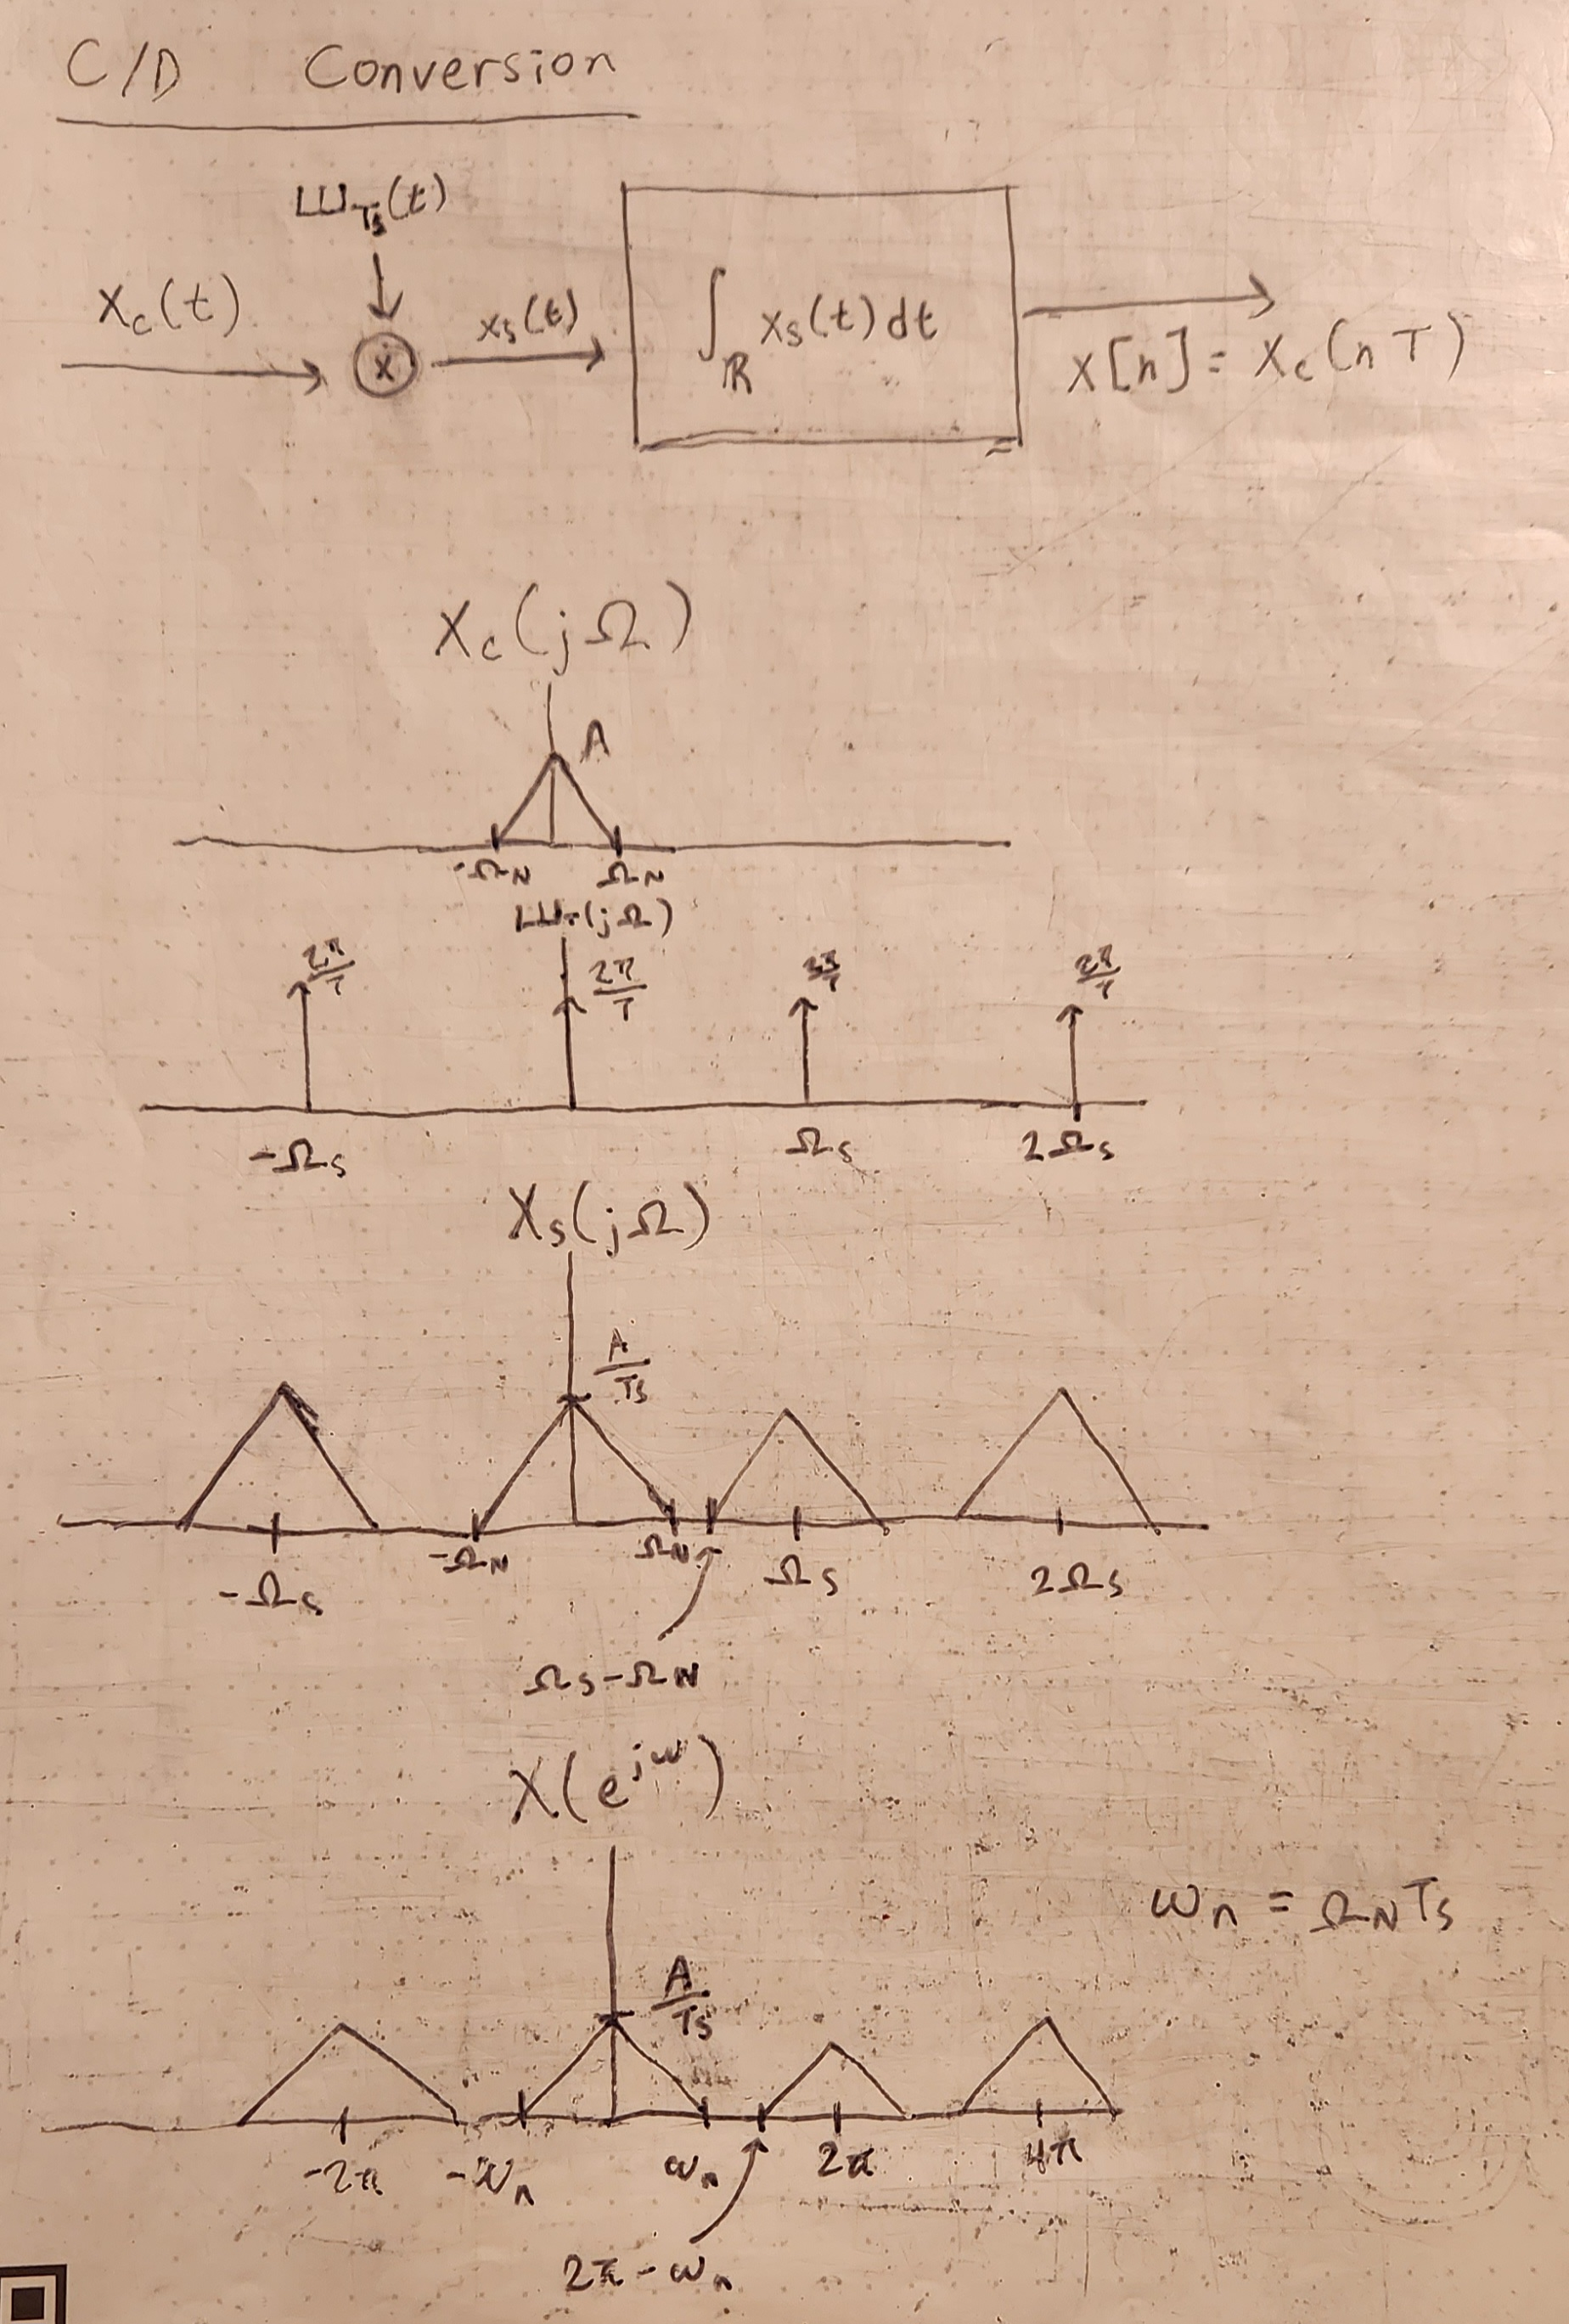
\includegraphics[scale=0.165]{graphics/cd_conversion.jpg}

  \pagebreak

  \subsubsection{D/C Conversion}

  \small\textbf{Mismatch in Reconstruction and Sampling Period}:

  Assuming no aliasing effects, if \(T_r \neq T_s\)

  \(y_r(t) = \dfrac{T_r}{T_s}x_c\prn{\dfrac{T_s}{T_r}t}\)

  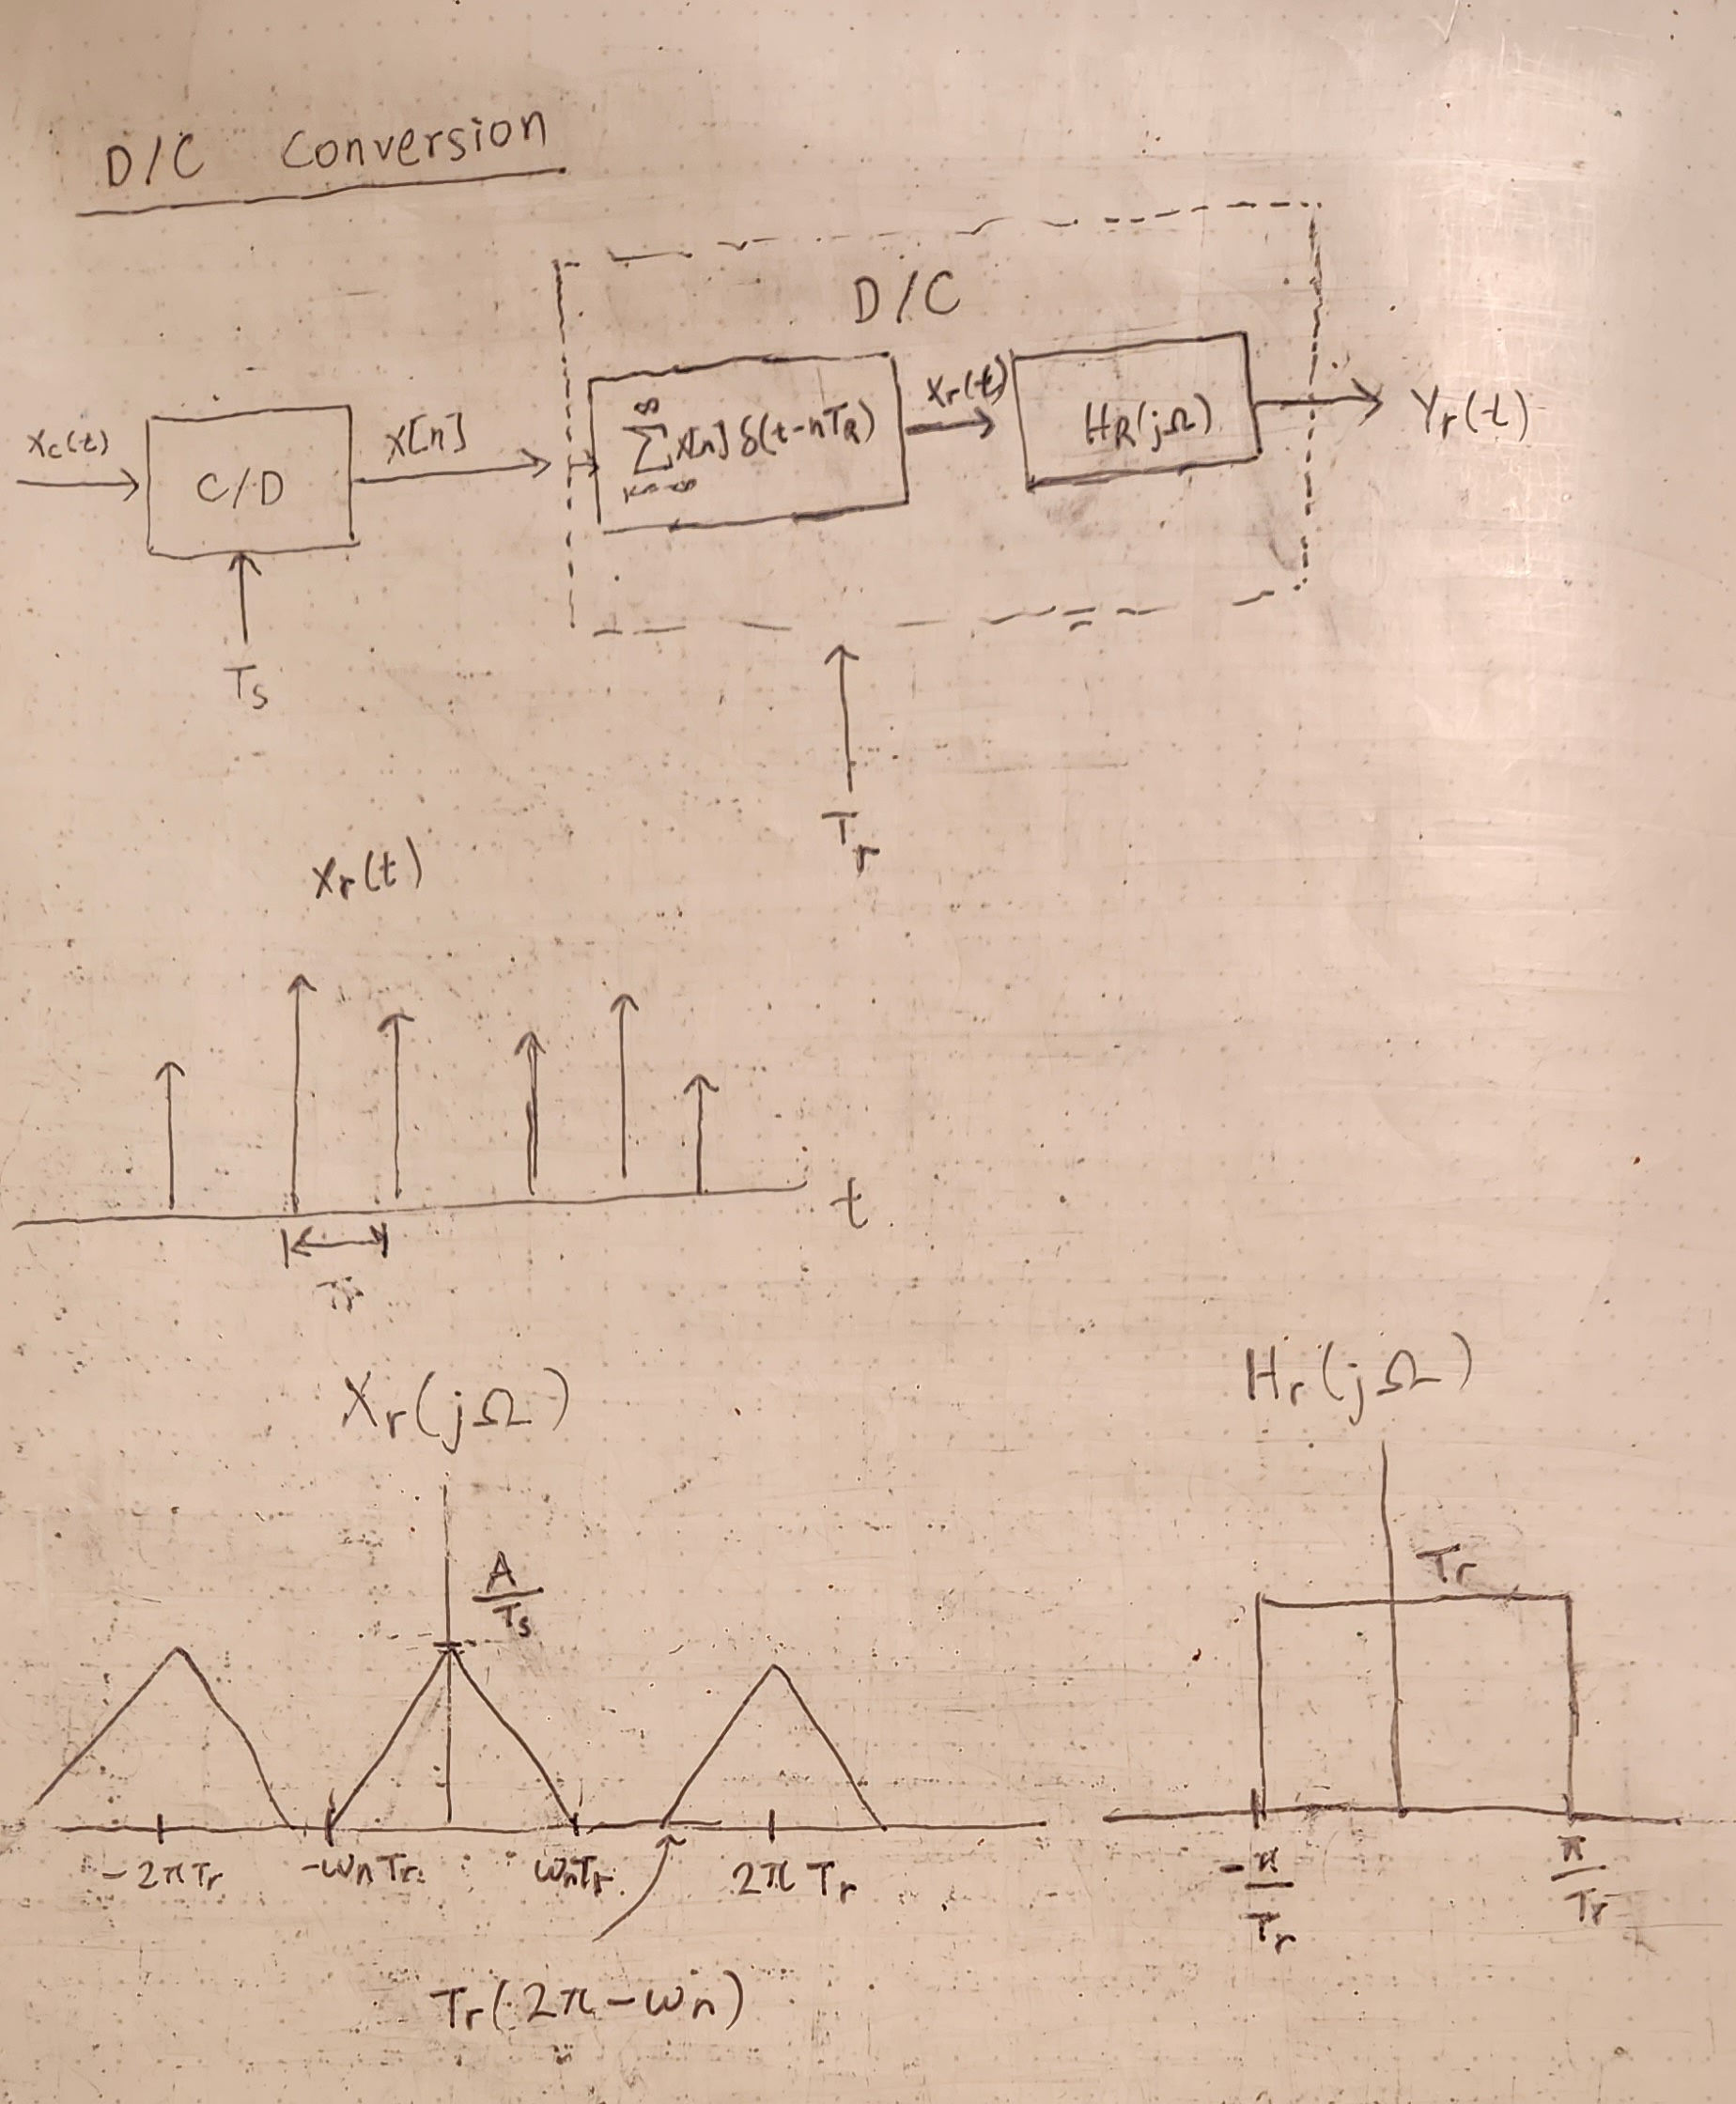
\includegraphics[scale=0.2]{graphics/dc_conversion.jpg}

  \pagebreak

  \subsubsection{Compression and Decimation}

  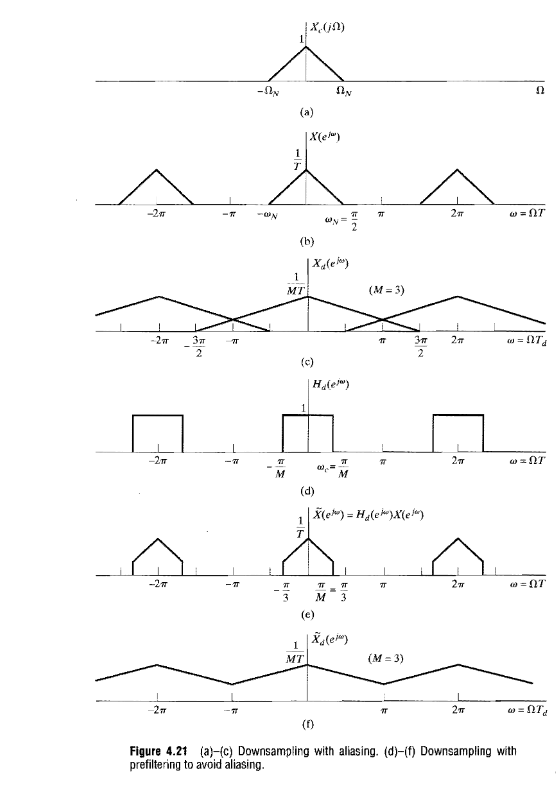
\includegraphics[scale=0.7]{graphics/downsampling.png}

  \pagebreak

  \subsubsection{Expansion and Interpolation}

  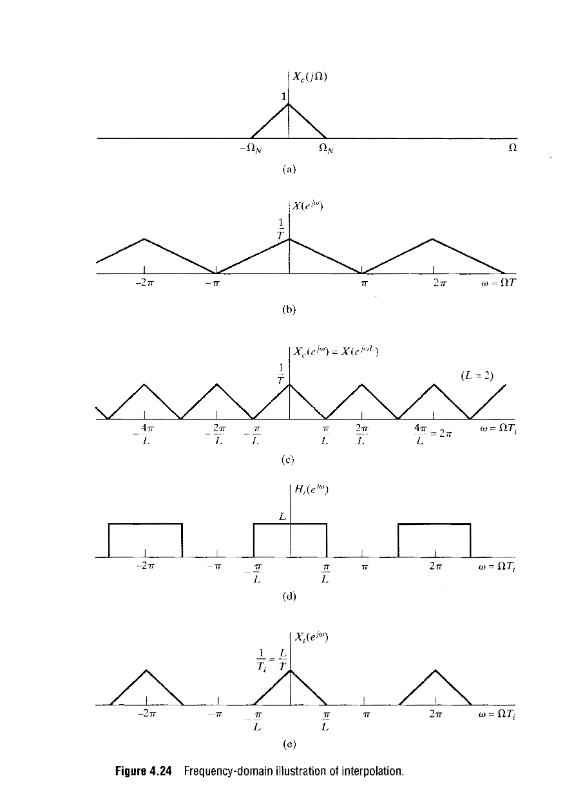
\includegraphics[scale=0.7]{graphics/upsampling.png}

  \pagebreak

  \subsubsection{Change Sampling Rate by Noninteger Factor}

  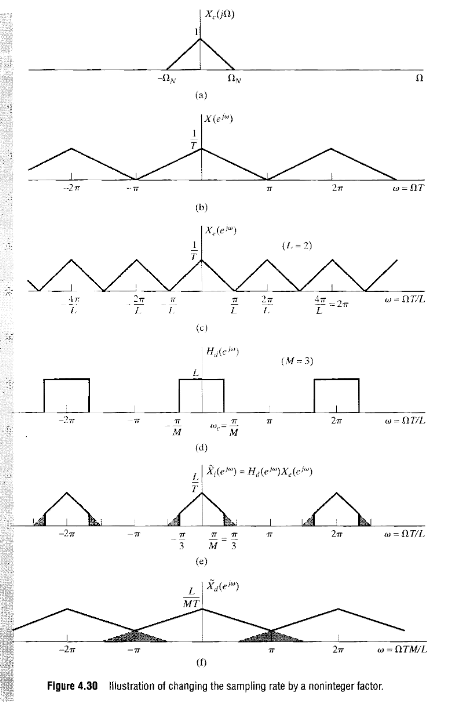
\includegraphics[scale=0.7]{graphics/noninteger.png}

  \pagebreak

  \subsubsection{Polyphase Decompositions}

  \textbf{Noble Identities:}

  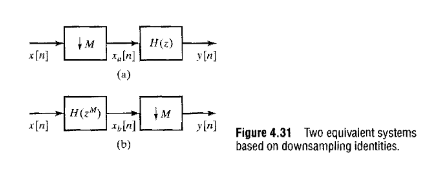
\includegraphics[scale=0.7]{graphics/compressor_noble.png}

  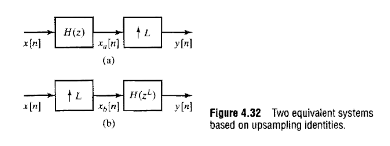
\includegraphics[scale=0.75]{graphics/expander_noble.png}

  \textbf{Polyphase Decomposition for Compression}:

  In the below diagram \(e_{k}[n] = h[nM + k]\)

  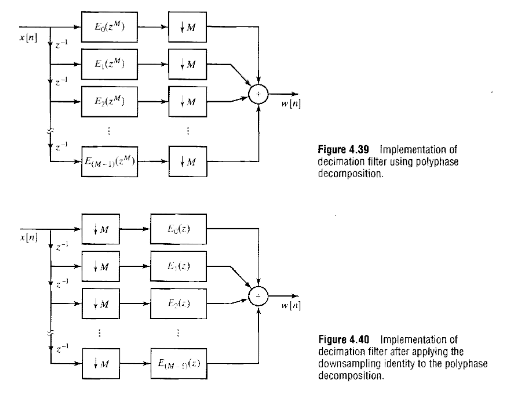
\includegraphics[scale=0.82]{graphics/polyphase_down.png}




\end{document}
